\documentclass[12pt,a4paper]{article}
\usepackage{amssymb}
\usepackage{fullpage}
\usepackage{graphicx}
\author{Parker Whaley}
\title{lab \#2}
\begin{document}
\maketitle
\section{Measured Data}
We first attempted to get the focal length of the two lenses.  While doing this we recorded two positions of each instrument each with a uncertainty of .1cm this gives the average an uncertainty of $\delta=.1/\sqrt{2}$.\\

We measured the position of the source as $ave(14.55cm, 18.45cm)=16.5cm \pm \delta$.\\

Next we set up our experiment to measure the focal lengths of the two lenses.  Below are the average distances (uncertainty $\delta$) to the mirror and the range of screen positions that focused $P_l$ to $P_h$.  We will not consider the uncertainty from the instrument's measurements for these last two as the uncertainty we had in where they focused is much higher as shown below (order of mm vs cm).\\

\begin{tabular}{| l | l | l | l | l | l |}
\hline
 & lens & $P_l$ & $P_h$ & $P$ & $\delta P$\\
\hline
L1 & 37.55 & 149.45 & 159.25 & 154.35 & 4.9\\
\hline
 & 42.9 & 97.625 & 101.375 & 99.5 & 1.875\\
\hline
L2 & 37.55 & 148.25 & 158.55 & 153.4 & 5.15\\
\hline
& 42.05 & 98.35 & 102.95 & 100.65 & 2.3\\
\hline
\end{tabular}\\

We then measured the distance to a virtual image.  To do this we calibrated the focus of a camera so that it focused in the range (59.675, 66.025).  Witch gives us a focus at $62.85\pm3.175$.  We then positioned the lens at various positions and measured the distance to the virtual image formed by lens one.  The range in these measurements is denoted $C_l$ to $C_h$.  Note that L has the previously described uncertainty $\delta$.\\

\begin{tabular}{| l | l | l | l | l |}
\hline
L & $C_l$ & $C_h$ & C & $\delta C$\\
\hline
17.45 & 59.575 & 65.525 & 62.55 & 2.975\\
\hline
22.45 & 53.575 & 61.775 & 57.675 & 4.1\\
\hline
27.45 & 40.875 & 48.975 & 44.925 & 4.05\\
\hline
\end{tabular}\\

Finally we positioned lens one near the source then lens two and finally the screen.  We set the positions of the lenses then experimentally determined the distance where the image on the screen came into focus.  All of the set measurements come with uncertainty $\delta$ the experimental value has experimentally determined uncertainty.\\

\begin{tabular}{| l | l | l | l | l | l |}
\hline
$L_1$ & $L_2$ & $S_l$ & $S_h$ & S & $\delta S$\\
\hline
32.3 & 52.3 & 71.8 & 72.55 & 72.175 & 0.375\\
\hline
23.05 & 58.9 & 86.95 & 87.85 & 87.4 & 0.45\\
\hline

\end{tabular}

\section{Lens behaviour}
Here I plotted $s_0^{-1}$ is the lens position minus the source position vs. $s_i^{-1}$ witch is the screen position minus the the lens position.\\
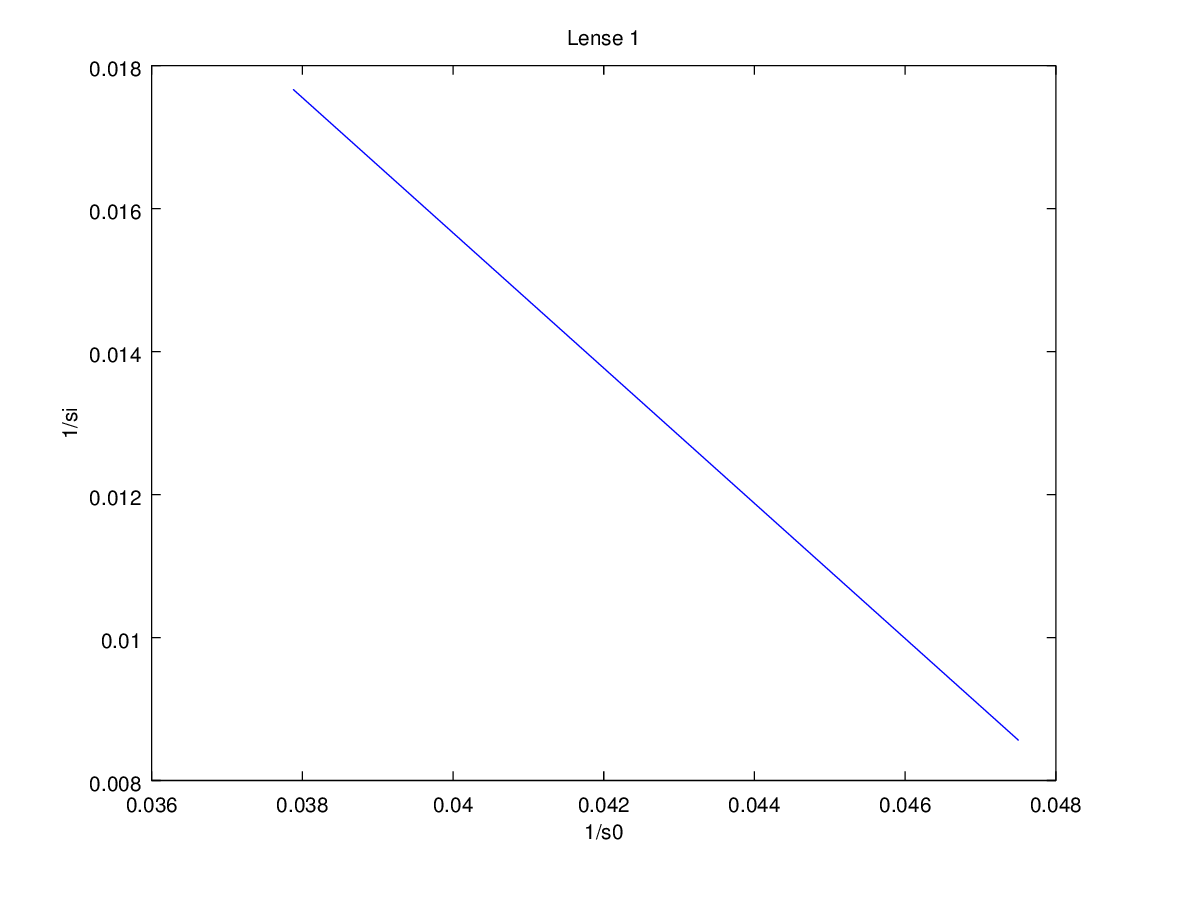
\includegraphics[scale=.7]{l1.png}\\
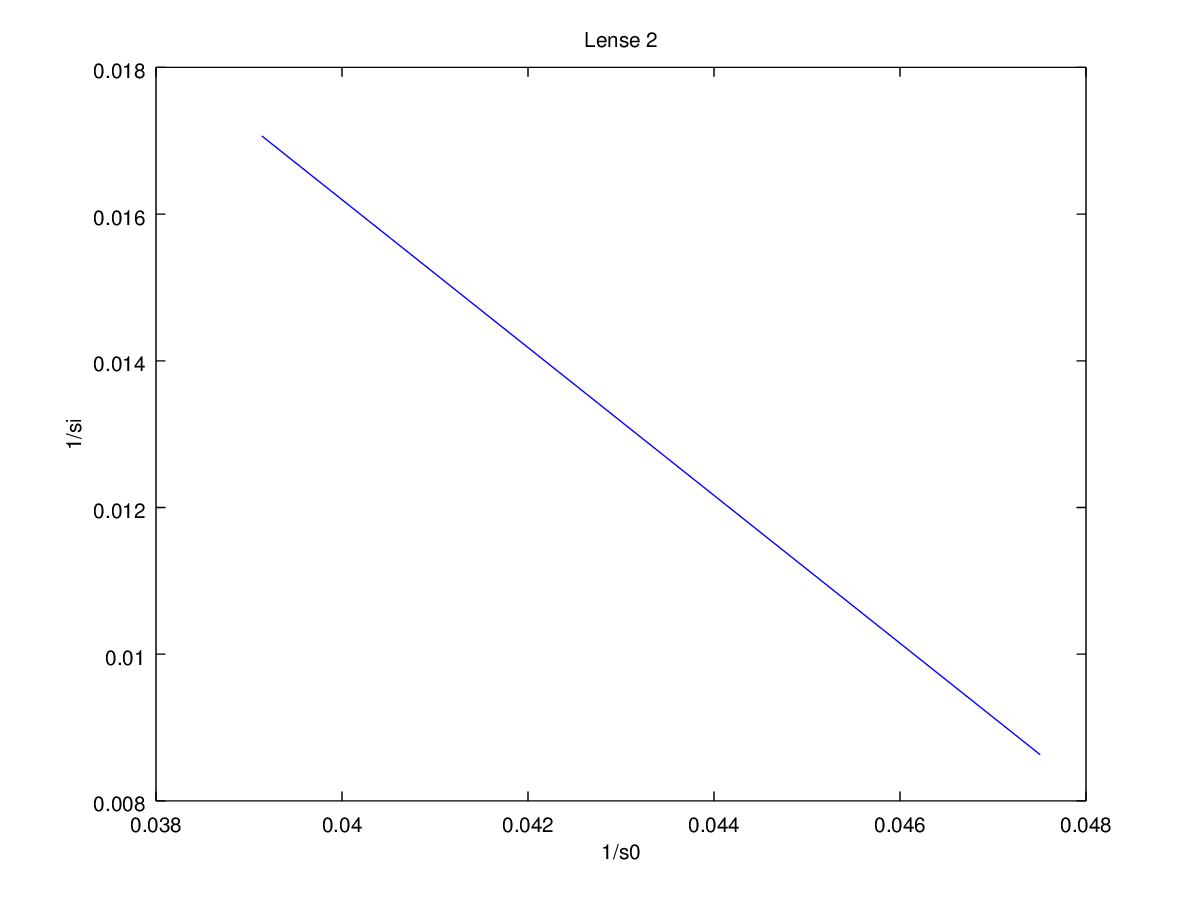
\includegraphics[scale=.7]{l2.png}\\

One point is not enough to get a line so I will instead do uncertainty analysis to get the focal length 
\[f=1/2((\frac{1}{L1-d}+\frac{1}{P1-L1})^{-1}+(\frac{1}{L2-d}+\frac{1}{P2-L2})^{-1})\]
Where d is the position of the source L (L1 and L2 describe the two separate measurements) is the lens position and P is the position of the screen. note that the uncertainty in everything except P is $\delta$ described above. Let us note that the uncertainties in everything other than P are so minuscule that they can be considered negligible, they are almost two orders smaller.  We then get:
\[\delta f^2=(1/2*\frac{1}{((\frac{1}{L1-d}+\frac{1}{P1-L1})(P1-L1))^2}*\delta P1)^2+(1/2*\frac{1}{((\frac{1}{L2-d}+\frac{1}{P2-L2})(P2-L2))^2}*\delta P2)^2\]
We then get $f_1=17.919 \pm 0.70711cm$ and$f_2=17.803\pm0.70711cm$.  These seem reasonable since in lab we eye balled the focal length at about 18cm.

\section{additional discussion}
These results seem physically reasonable, We were able to show that the focal length was a reasonable 17cm.  As discussed the errors were different for the two different measurements for each lens.



\end{document}